\documentclass[output=paper]{langsci/langscibook} 
\ChapterDOI{10.5281/zenodo.3975795}
\author{Henrik Bergqvist\affiliation{Stockholm University} \lastand Seppo Kittilä\affiliation{University of Helsinki}}

\title{Epistemic perspectives: Evidentiality, egophoricity, and engagement}
\shorttitlerunninghead{Epistemic perspectives}
% \title{\texorpdfstring{Word formation and word history:\\ The case of
%  \textsc{capitalist} and \textsc{capitalism}}{Word formation and word
% history:  CAPITALIST and
% CAPITALISM}}

% \renewcommand{\lsCollectionPaperFooterTitle}{Epistemic perspectives: evidentiality, egophoricity, and engagement}

 

\abstract{\noabstract}

\begin{document}
\maketitle

\section{Introduction}\label{s:hb1}
In the last decade, there has been a surge in output on various forms of epistemic marking in language, including (epistemic) modality, evidentiality, mirativity, egophoricity, and engagement.\footnote{Edited volumes that deserve mention are: \citeauthor{AikhenvaldDixon2003} (\citeyear{AikhenvaldDixon2003}; \citeyear{AikhenvaldDixon2014}) on evidentiality, modality, and expressions of knowing in grammar more broadly; \cite{GawneHill2017} on evidentiality in Tibetan languages and \cite{SanRoqueetal2018} on egophoricity. The list of journal articles on epistemic marking in grammar is (very) long, but we may note \citeauthor{Evansetal2017a} (\citeyear{Evansetal2017a}, \citeyear{Evansetal2017b}) on engagement, \cite{BergqvistKnuchel2017} on egophoricity, and \cite{SanRoqueetal2017} on evidentials and interrogativity.}
Some of these terms are better known than others.\footnote{By using terms like “evidentiality” and “egophoricity”, we refer to meaning domains that signal how knowledge about events can be qualified in different ways. Usually, such domain labels come with a definition that is found in the seminal literature dealing with a given domain (e.g. \citealt{Palmer2001}, for modality), but this is not always the case. Definitional criteria for comparable systems and forms are often contested and in a relatively young field such as the present one, debates concerning what counts as defining (semantic) features of a certain domain, are especially fierce. In this volume, a term like “evidentiality” is regarded as constituting a linguistic category in some languages, but consequently also refers to an epistemic domain that expresses different “modes of access” (\citealt{Plungian2010}) with respect to how knowledge about events may be acquired.} 
To begin with, epistemic modality has a long research tradition stemming from philosophy and qualifies an utterance in terms of possibility and probability, ranging from speculation to high certainty. The first monograph-length treatment of epistemic modality from a cross-linguistic perspective is \citeauthor{Palmer1986} (\citeyear{Palmer1986}; \citeyear{Palmer2001}). At about the same time, research on the related category, evidentiality, also began to gain momentum. Evidentiality signals the source of information that a speaker has for an utterance. It is often sub-divided into direct and indirect evidentials where direct evidentials target the (direct) perception of the speaker, signaling sensory access (visual, auditory) to a discourse object. Indirect evidentials express other types of cognitive access, such as inference, assumption, and hearsay, and may be differentiated by how directly accessible a given type of evidence is. For example, inference and assumption are both based on the speaker’s observation of a state-of-affairs that is not directly related to the event his/her claim is based on (e.g., we may infer that someone has left if that person’s coat is gone). Inference is usually based on direct sensory perception, while assumption is often based on our general knowledge of the world, thus differing in type of indirect access (see e.g. \citealt{Willett1988}). \citeauthor{Aikhenvald2004} (\citeyear{Aikhenvald2004}) is the first typological treatment of evidentiality, but it is \citeauthor{ChafeNichols1986}’ (\citeyear{ChafeNichols1986}) seminal volume that is commonly regarded as the first work to investigate evidentiality from a cross-linguistic perspective.
%%\isi{finality} 

Mirativity is regarded as separate from evidentiality by some (e.g. \citealt{DeLancey1997}), but the ultimate definition of this category (and even its existence) is still under debate.\footnote{See e.g. the debate in \emph{Linguistic Typology}, involving, among others, \cite{Hill2012}, \cite{DeLancey2012}, and \cite{HengeveldOlbertz2012}.}

Miratives signal new/non-assimilated knowledge and has often been said to convey the surprise of the speaker (\citealt{DeLancey1997}; cf. \citealt{Aikhenvald2014}). Surprise as a defining semantic component of mirativity has increasingly been rejected, however, whereas the signaling of new/non-assimilated information appears to be more widely accepted (but see \citealt{Hill2012} for arguments against the category of mirativity). In some languages (e.g. Turkish and Finnish), mirativity is found in specific uses of inferential evidential morphemes, while in other languages (such as Hare), there is a morpheme whose primary, or even only, function, is to signal mirativity (\citealt{DeLancey1997}).

Egophoricity signals the epistemic authority of a speaker or addressee (speech-act participant) subject to his/her involvement in a talked-about event (\citealt{Bergqvist2018b}; \citealt{BergqvistKittila2017}; cf. \citealt{Hargreaves2005}). This dialogical property of the egophoric marker has produced a pattern where egophoric markers occur in statements with first person subjects and in questions with second person subjects: \textit{I am leaving}. [\textsc{ego}] vs. \textit{Are you leaving?} [\textsc{ego}]. This functional overlap with person marking has led some to regard egophoric marking as a form of person marking/agreement, but it is clear from diachronic, distributional, and semantic criteria that egophoric marking is distinct from person marking (see \citealt{BergqvistKittila2017}, for a discussion). Egophoricity, as a term to designate this kind of epistemic marking, was proposed by \citeauthor{Tournadre1996} (\citeyear[201]{Tournadre1996}), but the forms he discussed using the term had already been described by Austin \cite{Hale1980} for Kathmandu Newar, then called “conjunct” (contrasted to “disjunct”). Subsequent research on the phenomenon called into question the usefulness of the label “conjunct/disjunct” and various proposals were put forth to replace it (e.g. “assertors involvement”, \citealt{Creissels2008}; “congruent/non-congruent”, \citealt{Dickinson2000}). \cite{SanRoqueetal2018} opts for the term ``egophoricity'' in providing a comprehensive overview of the phenomenon.

``Engagement'', finally, is a term that has had some currency in French linguistics (e.g. \citealt{Descles2009}; \citealt{Guentcheva2011}) and in discourse studies (\citealt{Hyland2005}), but in the work of \citeauthor{Evansetal2017a} (\citeyear{Evansetal2017a}, \citeyear{Evansetal2017b}) it is used as a label for a kind of epistemic marking separate from the categories outlined above. Engagement targets the epistemic perspectives of the speech-act participants, signaling differences in the distribution of knowledge and/or attention between the speaker and the addressee. As such, it specifies whether information is shared, or exclusive to one of the speech-act participants. This contrast is exemplified with data from Southern Nambikwara (\citealt[63--64]{Kroeker2001} [our adjusted glossing and translation]):

\begin{exe}
\ex Nambikwara \label{ex:hb1}
	\begin{xlist}
	\ex 
	\gll wa3ko3n-a1-\textbf{Ø}-wa2.\\
	work-1-\textsc{prs}-\textsc{excl}-\textsc{impf}\\
	\trans ‘I am working.’ 
	\ex 
	\gll wa3ko3n-a1-\textbf{ti2.tu3}-wa2\\
	work-1-\textsc{shrd}-\textsc{impf}\\
	\trans ‘(You and I see that) I am working’ 	
	\end{xlist}
\end{exe}

In (\ref{ex:hb1}), the semantic contrast between exclusive and shared knowledge is signaled by a zero morpheme and the -\textit{ti2.tu3}-suffix, respectively.\footnote{\citeauthor{Kroeker2001}’s label for what we term engagement, is ``verification”.}

While the translation suggests a visual mode of access to go along with such knowledge asymmetry, this is not encoded in said forms, but signaled by means of separate evidential morphology (see \citealt{Kroeker2001}, for details).
Engagement markers are generally underspecified with respect to how knowledge about an event is gained, but \cite{Evansetal2017b} note that engagement markers often combine with evidentials and modals to signal (a)symmetries in terms of accessibility to and belief of some event. An issue that relates to the topic of the present volume in terms of categorical overlap, is whether the assumed distribution of knowledge between the speech-act participants concerns their actual knowledge/non-knowledge, or their rights/non-rights to knowledge (see \citealtv{chapters/02_grzech}).
It is possible that this contrast in terms of knowledge access and rights to knowledge is subject to variation across engagement systems. While engagement has yet to be widely accepted as a grammatical category in some languages, arguments for making such a claim are put forth in §\ref{s:hb3-3}, below. 

The organization of this introductory chapter is as follows: In §\ref{s:hb2}, we will discuss the functional and semantic overlaps between the discussed categories on a general level. In §\ref{s:hb3}, we will focus on the relation between the discussed categories as resources for expressing epistemic authority, and in §\ref{s:hb4}, we will summarize the main points of the paper and suggest some ideas for future research.

\section{Functional and semantic overlap between categories}\label{s:hb2}
 
It is a widely known fact that the abovementioned categories overlap in form, meaning, and function (see \citealt{Cornillie2009}; de \citealt{Haan1999}; \emph{inter alia}). This has been especially noted with respect to modality and evidentiality, where an English modal verb like \emph{must} may be treated as a modal, or an evidential depending on the context of use. Such ambiguity has led some researchers to analyze evidentiality as a subtype of modality (e.g. \citealt{Palmer1986}; \citealt{Palmer2001}), whereas others have argued for a strict separation between the two categories (e.g. \citealt{Aikhenvald2004}).

A comparable overlap has also been observed for evidentiality, mirativity, and egophoricity. With respect to evidentiality and mirativity, an inferential (evidential) form may also serve as a mirative depending on the context of use, as in Turkish (\citealt{SlobinAksu1982}). Evidentiality and egophoricity overlap to the extent that egophoric markers may be part of evidential paradigms and thus contrast with evidential forms. Semantically, some have argued that egophoric marking cannot be regarded as a kind of evidential marking due to the fact that such markers do not signal a source of information as such (e.g. \citealt{Aikhenvald2004}). Others have argued the opposite and regard egophoric markers as the strongest kind of access that speakers employ to justify a statement (\citealt{Plungian2010}; \citealt{SanRoqueLoughnane2012}; cf. \citealt{Boye2012}, evidentiality as ``justification''). Egophoric markers have sometimes been analyzed as a kind of mirative marker for Tibetan and Barbacoan languages (\citealt{DeLancey1997}; \citealt{Dickinson2000}; but see \citealt{Curnow2002b}, for a critique). \citeauthor{Kittila} (forthcoming), shows that egophoric markers have features in common with general knowledge/factual evidentials and that claims of factuality may formally resemble markers of both visual evidence and volitional participation in an event.

Several papers in this volume discuss categorical overlaps of the kind sketched above. We will mention a few of them here. Liljegren notes for the Indo-Aryan language Palula that indirect evidentiality is produced by the contextualized token-use of perfect forms in addition to employing sentence final particles denoting hearsay and inference. The use of aspectual forms and particles to serve evidential functions are a commonly noted phenomenon, which has also been attested for Turkic (\citealt{SlobinAksu1982}), Caucasian (\citealt{Tatevosov2001}), and Persian languages (\citealt{Lazard1996}).

Grzech accounts for epistemic markers in a variety of Quechua that previously have been described as evidentials, but which Grzech analyzes as signaling epistemic authority. Given the defining role of epistemic authority in egophoric marking, this constitutes a clear case of conceptual overlap between the two categories where a set of evidential markers (i.e. that are cognate to evidentials in related languages) have developed egophoric semantics. While assigning epistemic authority is implied by the use of direct and indirect evidentials (see §\ref{s:hb3-1}, below), it has become encoded in Tena Kichwa, an Ecuadorian variety of Quechua. Conversely, languages with egophoric marking (see e.g. \citealt{Tournadre2008}) may imply the cognitive access that a speaker claims for making an assertion, while the speaker’s epistemic authority is encoded in the form (see §\ref{s:hb3-2}, below).

For Kalapalo, Basso accounts for an enormously rich variety of epistemic markers with different grammatical status that includes modal and evidential notions, but which also feature participation and the positioning of knowledge between the speech-act participants. In a language like Kalapalo, it may not be fruitful to base categorical distinctions on formal criteria, given their distribution in different parts of the grammar. Rather than a small number of forms serving many functions, Kalapalo has many forms serving overlapping functions, thus constituting an entirely different kind of categorical overlap than the one that e.g. Liljegren reports for Palula.
%
\section{The relation between evidentiality, egophoricity, and engagement}\label{s:hb3}

How may we account for the overlaps discussed above? The conceptual overlap between categories is evident from a functionalist perspective, but how this corresponds to their semanto-pragmatic properties and distinct development requires further discussion. With respect to the development of markers belonging to the categories that are the topic of the present volume, it is clear that the presence of pragmatically contingent components of meaning (e.g. inference as a token-feature of perfects) makes possible an eventual encoding of this implied feature to become part of the semantics of a form. This conventionalization of implicature (\citealt{Levinson2000}) is a driving force in grammaticalization processes more generally and we may observe this for epistemic marking, as well (see \citealt{Bergqvist2018b}). The aim of this section is to account for how implied meaning in the use of certain markers suggests the relation between the investigated categories and the reason for the frequently attested overlaps between categories.
%
\subsection{Cognitive access vs. (dis)claiming epistemic authority: Evidentiality}\label{s:hb3-1}

The notion of evidentiality in language has been equated with providing justification for how information was acquired, i.e. the source of information that a speaker has for making an assertion about an event. \cite{Willett1988} is still a good starting point for an illustration of the basic semantic features and divisions relevant to evidentiality in a cross-linguistic sense. 

%%TODO table 1
\begin{figure}
    \centering
%     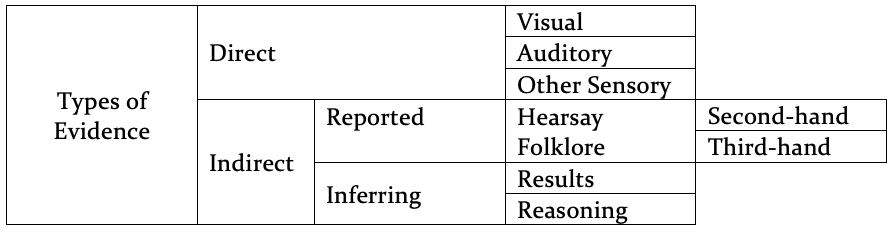
\includegraphics[width=\textwidth]{figures/bergqvist-fig1.png}
    \begin{forest}  for tree={
    grow'=0,
    child anchor=west,
    anchor=west,
  }
[types of evidence
    [direct
        [visual]
        [auditory]
        [other sensory]
    ]
    [indirect
        [reported
            [\parbox{1.2cm}{hearsay\\folklore}
                [second-hand]
                [third-hand]
            ]
        ]
        [inferring
            [results]
            [reasoning]
        ]
    ]
]
\end{forest}
    \caption{Evidential categories (after \citealt{Willett1988})}
    \label{fig:my_label}
\end{figure}


There is an implicit expectation for the speaker to provide the highest form of evidence for an assertion, which produces a hierarchical relation in terms of strength of evidence. Direct evidentials conveying ``visual'' access (i.e. ‘I know this from having seen it’) usually constitutes a stronger form of evidence than other sensory access (i.e. ‘I know this from having heard/felt/smelt it’). It is, however, important to note that states-of-affairs display variation in this regard. For example, olfactory evidence is more direct and reliable for a claim like ‘There must be a gas leak here somewhere’, and tactile evidence outranks visual evidence for claims such as ‘The water is hot’. In general, though, visual evidence ranks highest, a suggestion that is supported by the use of visual evidential forms to express participatory/factual evidence in some languages (see §\ref{s:hb3-2}, below). For indirect evidentials, it is possible to argue that making an inference based on e.g. visual evidence (i.e. ‘I know this because I know/see what caused it’) is a stronger form of assertion than one based on report (i.e. ‘I know this because someone told me about it’). As stated above, inference and assumption are in principle very similar types of evidence, and both of them are classified as personal and indirect evidence by \cite[37]{Plungian2010}. 
However, these two evidence types differ from each other as regards their directness and reliability; inference is based on a more reliable (usually directly observable) evidence, while assumption is based on our general knowledge of the world (see the definitions offered by \citealt[37]{Plungian2010}). We can also see that the hierarchical relation between direct and indirect evidence in terms of strength may not always hold, since e.g. “folklore”, as a kind of reported evidential (i.e. ‘I know this from (our) oral tradition’), may be deemed a very reliable source despite the fact that no member of the speech community has direct access to the events portrayed. 

Possibly the most thoroughly investigated aspect of evidentiality is reported speech,\footnote{This is an impressionistic claim that would be difficult to substantiate statistically given the (by now) vast literature on evidentiality. Reportive evidentials were, however, discussed as early as \cite{Jakobson1957} and has continued to occupy research on European languages as well as more cross-linguistically oriented research (see e.g. \citealt{Boye2012}).} which also corresponds to the “simplest” kind of evidential system where reported speech is the only evidential marker. Estonian exemplifies such a system with only a hearsay marker (see \citealt{Aikhenvald2004} for details). But despite this emphasis on reported speech in the literature on evidentiality, a narrow conception of evidentiality as a verbal category tends to emphasize the role of direct perception (i.e. visual, auditory) in grammaticalized evidentiality systems. In \citeauthor{Haan2013}’s (\citeyear{Haan2013}) survey of evidential systems, however, systems that feature both direct and indirect evidentials are much less common than systems with only indirect evidentials. Evidential systems with only \emph{direct} evidentials are not attested at all in the survey. From this cross-linguistic patterning, we may gather that the grammatical expression of evidentiality is primarily a means to signal indirect access to events, and that this indirect access sometimes is (explicitly) contrasted to direct access. In the default case (i.e. indirect access to an event), evidentiality is not so much a strategy to signal ownership of knowledge through some cognitive channel, but a disclaimer of epistemic authority as a consequence of restricted (i.e. indirect) sensory access (cf. \citealt{Mushin2001}). 

Signaling indirect access to an event in terms of inference, or assumption, does not necessarily mean that there is a restriction present on the sensory access that a speaker has to the talked-about event. In data resulting from the use of an interactive elicitation task developed by Nick Evans and colleagues (described in \citealt{SanRoqueetal2012}), it is clear that explicit, visual representations of people, things, and events will prompt the use of inferentials and assumptives even in cases where such representations appear unambiguous (e.g. \citealt{Quartararo2017}). The simple fact that depicted events and people are outside of the speaker’s domain of epistemic authority, may be sufficient to warrant a more cautious approach to asserting such events by using indirect evidentials. The speaker may mark an event as being inferred from his/her point of view, rather than claiming direct perceptual access to the contents of the picture, possibly because such contents pertain to previously unknown characters in a fictional universe. 
\cite{Curnow2003} discusses the use of non-visual/indirect forms with first person subjects to produce unintentional/non-volitional readings of utterances (see Example \ref{ex:hb2b}, below). Such interpretation effects are in line with the hypothesis that indirect evidentials function as disclaimers of epistemic authority. However, it is also possible to use evidentials to \emph{claim} epistemic authority by means of direct evidentials. This may be a less prominent function of evidentials, but one that links evidentiality to egophoricity (see §\ref{s:hb3-2}, below). Just like indirect evidentials may be used even in cases where the speaker has direct sensory access to a talked about event, so are direct evidentials sometimes used to signal other forms of access than their semantics may suggest (i.e. visual, auditory). One such form of access that may be signaled by the use of direct evidentials, is “(volitional) participation”. Participatory meaning in the context of evidentiality may result from the distribution of direct evidential forms with subject pronouns (i.e. first vs. third person), or they can constitute distinct forms that are part of paradigms alongside other direct forms that signal visual access to the referent (see Example \ref{ex:hb3}, below). Examples of how the distribution of direct evidentials may produce participatory meaning according to subject person, is discussed by \citeauthor{Curnow2002b} (\citeyear[188--190]{Curnow2002b}, citing \citealt[133]{Ramirez1997}): 

\begin{exe}
\ex Tucano\label{ex:hb2}
	\begin{xlist}
	\ex \label{ex:hb2a}
	\gll bapá bope-ápɨ\\
	plate break-\textsc{rec}.\textsc{past}.\textsc{non}3.\textsc{visual}\\
	\trans ‘I broke the plate (of my own will, e.g., because I was angry).’ 
	\ex \label{ex:hb2b}
	\gll bapá bope-ásɨ \\
	plate break-\textsc{rec}.\textsc{past}.\textsc{non}3.\textsc{nonvisual}\\
	\trans ‘I broke the plate accidentally (I didn't see it on the table).’ 	
	\end{xlist}
\end{exe}

Curnow discusses the examples from Tucano as an instance of interpretation effects resulting from the distribution of forms signaling a visual/non-visual contrast with first person subjects. Such effects are also reported for other languages and depending on what evidentials are present in each language, different effects may arise (see \citealt{Curnow2002b}; \citeyear{Curnow2003} for details).

In Central Pomo, the evidential paradigm contains a form, -\textit{la}, which denotes “personal agency” (\citealt[181]{Mithun1999}):

\begin{exe}
\ex Central Pomo\label{ex:hb3}\\
	\gll da-ché-w=la\\
	pulling-seize-\textsc{prf}=\textsc{personal}.\textsc{agency}\\
	\trans `I caught it.’ (I know because I did it) 
\end{exe}

It should be noted that performative, or participatory, evidentials assume part of the function of person agreement, given the implied agency of a first person subject in such forms. Subject identity is not an encoded feature, however, and reference to the actions of third person subjects featuring performative/participatory forms may produce a factual reading that corresponds in epistemic status to participatory meaning when referring to events and actions involving the speaker. This means that factual events involving third persons may be marked in the same way as events involving one of the speech-act participants as a participant. \citeauthor{BergqvistKittila2017} (\citeyear{BergqvistKittila2017}; cf. \citealt{Bergqvist2015}) explores participation/involvement as part of evidential systems in order to place this notion against egophoric marking, in which volitional participation/involvement has been suggested as a defining notion (see directly below). One reason to make such a comparison relates to the ongoing debate on whether egophoric marking is a kind of evidential marker, or if egophoric marking constitutes a separate grammatical expression altogether. If “source of information” (\citealt{Aikhenvald2004}) is the preferred definition, then participation will be difficult to accommodate within such a definition (but see \citealt{SanRoqueLoughnane2012} for a discussion). If viewed from the perspective of epistemic marking in language, more generally, then cognitive access to events must be situated against related means to signal access more broadly, including access from participation/involvement (see \citealt{Bergqvist2017}; cf. \citealt{Boye2012}).  
%
\subsection{Involvement and epistemic authority: Egophoricity}\label{s:hb3-2}

Egophoricity is a recently proposed term for a form of epistemic marking that prototypically occurs with first and second person subjects in declarative and interrogative clauses, respectively (see \citealt{SanRoqueetal2018}, for a cross-linguistic overview). Egophoricity is also known as “conjunct/disjunct”-marking in the literature (e.g. \citealt{BickelNichols2007}), but competing terms also exist (see §\ref{s:hb1}, above). Example (\ref{ex:hb4}) portrays the two combinations of subject person and sentence type that trigger egophoric marking in Kathmandu Newar (\citealt{Hale1980}). All other combinations of subject person and sentence-type produces non-egophoric marking (i.e. 1S+interrogative/2S+declarative/3S+any sentence type):

\begin{exe}
\ex Kathmandu Newar (\citealt[95]{Hale1980}, [our adjusted glossing]) 
\label{ex:hb4}
	\begin{xlist}
	\ex 
	\gll ji	ana	wanā\\
	1\textsc{s}.\textsc{abs} there go.\textsc{ego}\\
	\trans ‘I went there.’ 
	\ex 
	\gll cha ana wanā lā \\
	2\textsc{s}.\textsc{abs} there go.\textsc{ego} \textsc{interr}\\
	\trans ‘Did you go there?’ 	
	\end{xlist}
\end{exe}

In addition to this distributional pattern, there are also restrictions on what verbs may take the egophoric marker. In Kathmandu Newar, only verbs that feature (volitional) agents are permitted. The contrast between verbs that denote volitional actions and ones that do not, is illustrated in (\ref{ex:hb5}) (\citealt[12--13]{Hargreaves2005}):

\begin{exe}
\ex Kathmandu Newar\label{ex:hb5}
	\begin{xlist}
	\ex 
	\gll jĩ:	jyā	yān-ā\\
	1.\textsc{erg} work	do-\textsc{pst}.\textsc{ego}\\
	\trans ‘I did the work.’ 
	\ex 
	\gll ji mhiga then-a\\
	1.\textsc{abs} yesterday arrive-\textsc{pfv}.\textsc{allo}\\
	\trans ‘I arrived yesterday.’ 	
	\ex 
	\gll jĩ:	thul-a\\
	1.\textsc{erg} understand-\textsc{pfv}.\textsc{allo}\\
	\trans ‘I understood (it).’ 
	\end{xlist}
\end{exe}

\cite{BergqvistKnuchel2017} take a broad approach to analyzing egophoric marking by outlining the boundaries of speech-act participant involvement in such systems. Although the volitional actions of a speech-act participant purportedly are a defining semantic component of egophoric marking, it has become increasingly clear that this is not the only kind of involvement that may trigger the use of an egophoric marker. Involvement as a basis for epistemic authority may in some instances target the affectedness, or even the attitude of a speaker/addressee (\citealt[369]{BergqvistKnuchel2017}). Given that such an encompassing formulation of involvement is applicable to some egophoric markers, \citeauthor{BergqvistKnuchel2017} propose that “epistemic authority” is actually the core semantic notion that may define egophoric marking against other forms of epistemic marking, such as evidentials and epistemic modals. Focusing on the notion of epistemic authority also bridges the gap to seemingly unrelated phenomena such as “ethical datives”, which share formal and functional features with egophoric marking, as described for a language like Standard Tibetan (see \citealt{BergqvistKnuchel2017}, for details). The involvement of a speech-act participant produces a kind of epistemic inalienability that permits the speaker to assign epistemic authority to him/herself, or the addressee without necessarily specifying what this involvement consists of.

The notion of epistemic authority may be conceptualized as a driving force in verbal interaction more generally and serves to situate information with respect to the speech-act participants. As such, it goes well beyond the use of egophoric markers in languages where this is an attested form of epistemic marking. For English (arguably a language without egophoric marking), the notion of epistemic authority may be seen in the correspondence between sentence-type and communicative function, an issue that has concerned speech-act theory since its formulation (\citealt{Searle1969}). Sometimes an assertion may function as a question in a communicative sense, and vice versa. In fact, the majority of polar questions in American English have the form of an assertion (\citealt{Stivers2010}; \citealt{StiversRossano2010}). In order to explain this apparent discrepancy, \cite{Heritage2012} argues that the notions, “epistemic status” and “epistemic stance” are key for understanding discrepancies between grammatical form and (social) action. Epistemic status, as an index of relative epistemic authority, is formulated with reference to the notion of A and B-events (\citealt{Labov1977}), where A-events are known only to the speaker (speaker authority) and B-events are known only to the addressee (addressee authority). Typical B-events include the addressee’s opinions, beliefs, and bodily states, but may also include his/her professional expertise. Heritage offers the following definition of epistemic status:

\begin{displayquote}
	(W)e can consider relative epistemic access to a domain as stratified between actors such that they occupy different positions on an epistemic gradient (more knowledgeable [K+] or less knowledgeable [K−]), which itself may vary in slope from shallow to deep […]. We will refer to this relative positioning as epistemic status, in which persons recognize one another to be more or less knowledgeable concerning some domain of knowledge (…) (\citealt[32]{Heritage2012})
\end{displayquote}


The speaker's epistemic stance can be congruent or incongruent with the speaker’s epistemic status, as seen in the example, \emph{you’re married}, provided by \citeauthor{Heritage2012}, which may be understood as a request for confirmation despite its assertive formulation, given that it pertains to the addressee’s marital status. A statement such as, \emph{you’re sad}, using an assertive form, may be deemed incongruent to the speaker’s epistemic status, given that it must be regarded as K-, given the addressee’s obvious epistemic authority over his/her own emotional states.

Speakers of any language continuously keep track of what others know and how their own knowledge can be related to the knowledge of others, and \citeauthor{Heritage2012} offers us a detailed and empirically grounded picture of how this works in everyday conversation. Such assumptions most prominently involve the addressee and explicit formulations of how the addressee’s perspective is attended to have received some attention in the field of discourse studies, notably in work by Ken \citeauthor{Hyland1999} (e.g. \citeyear{Hyland1999}; \citeyear{Hyland2001}; \citeyear{Hyland2005}). More recently, cross-linguistic research has led to the formulation of “engagement” as a bona fide epistemic category in some languages (see \citealt{Evansetal2017a}) and the relation between engagement and epistemic authority deserves to be explored in the definition of both notions.

\subsection{Shared vs. non-shared access/rights to knowledge: Engagement}\label{s:hb3-3}

Engagement consists of a contrast between the speaker’s assertion about the addressee’s knowledge of/attention to an event (\textit{e}) as either \emph{shared} or \emph{non-shared} with the speaker. \emph{I know e and I assume that you know e too}, is contrasted with, \emph{I know e and I assume that you do not} (\citealt{Evansetal2017a}; cf. “complex perspective”, \citealt{Evans2005}; cf. “complex epistemic perspective”, \citealt{Bergqvist2015,Bergqvist2016}; \citeyear{Bergqvist2017}). This semantic contrast may in principle concern any aspect of epistemicity, and is as such relevant for any form of epistemic marking (see below). Engagement targets “knowing” from a socio-centric perspective, where the speaker’s assertion contains an embedded assertion assumed to belong to the addressee. Such assumptions may be implied in the token-use of other forms of epistemic marking, but in a language with engagement as a category, this implicature has become encoded in forms to signal asymmetries in the knowledge/attention states of the speech-act participants.


In Kogi (Arwako-Chibchan; \citealt{Bergqvist2016}; cf. \citealt{Ortiz1994}), speakers can choose one of four auxiliary prefixes that encode engagement.\footnote{\citeauthor{Bergqvist2015} (\citeyear{Bergqvist2015}; \citeyear{Bergqvist2016}; \citeyear{Bergqvist2017}) discusses the Kogi system using the term “complex epistemic perspective” without arguing for a more general applicability of this term to similar systems and forms in the literature. Such applicability is, however, considered in \citeauthor{Evansetal2017a} (\citeyear{Evansetal2017a}, \citeyear{Evansetal2017b}) under the term engagement.} 
These prefixes may be divided into two sets that take the speaker and the addressee as their respective starting points. A focus on the perspective of the speaker is found with \textit{na-}/\textit{ni-}, where \textit{na-} means that ‘the speaker knows \textit{e} and expects the addressee to be unaware of \textit{e}’ (\ref{ex:hb6a}), and \textit{ni}- means that ‘the speaker knows \textit{e} and expects the addressee to know \textit{e} too’ (\ref{ex:hb6b}) (\citealt[2]{Bergqvist2016}):

\begin{exe}
\ex Kogi\label{ex:hb6}
	\begin{xlist}
	\ex \label{ex:hb6a}
	\gll kwisa-té	\textbf{na}-nuk-kú\\
	dance-\textsc{impf}	\textsc{spkr}.\textsc{asym}-be.\textsc{loc}-1\textsc{s}\\
	\trans ‘I am/was dancing.’ (informing) 
	\ex \label{ex:hb6b}
	\gll kwisa-té	\textbf{ni}-nuk-kú\\
	dance-\textsc{impf}	\textsc{spkr}.\textsc{sym}-be.\textsc{loc}-1\textsc{s}\\
	\trans ‘I am/was dancing.’ (confirming)  
	\end{xlist}
\end{exe}

\textit{Na}-/\textit{ni}- are in turn contrasted to \textit{sha}-/\textit{shi}-, which encode a corresponding distinction in terms of non-shared/shared knowledge from the addressee’s perspective. \textit{sha}- means that ‘the speaker expects the addressee to know \textit{e} while the speaker is unaware of \textit{e}’ (\ref{ex:hb7a}), and \textit{shi}- means that ‘the speaker expects the addressee to know \textit{e}, and the speaker knows \textit{e} too’ (\ref{ex:hb7b}) (\citealt[3]{Bergqvist2016}):


\begin{exe}
\ex Kogi\label{ex:hb7}
	\begin{xlist}
	\ex \label{ex:hb7a}
	\gll nas	 hanchibé \textbf{sha}-kwísa=tuk-(k)u\\
	1\textsc{sg}.\textsc{ind}	good \textsc{adr}.\textsc{asym}-dance=be.\textsc{loc}-1\textsc{sg}\\
	\trans ‘I am dancing well(?)’ (in your opinion) 
	\ex \label{ex:hb7b}
	\gll kwisa-té	\textbf{shi}-ba-lox\\
	dance-\textsc{impf}	\textsc{adr}.\textsc{sym}-2\textsc{sg}-be.\textsc{loc}\\
	\trans ‘You are/were dancing(?)’ (confirming)  
	\end{xlist}
\end{exe}

\textit{Shi}-/\textit{sha}- are used to signal the speaker’s acknowledgement of the addressee as primary knower, but at the same time encodes the speaker’s assertion (without reduced certainty) of a talked about event. 

Engagement in Kogi may appear to be an exotic system in a little-known language, but this notion echoes with well-known phenomena like modal particles in Germanic languages (modal particle). Descriptive accounts of cognates of the German \textit{ja} (‘as you know’/`of course’, \citealt{Abraham1991}), in Danish (\textit{jo}, \citealt{Davidsen1996}), Norwegian (\textit{jo}, \citealt{Andvik1992}) and Swedish (\textit{ju}, \citealt{Lindstrom2008}) agree that reflexes of this form signals “available knowledge through shared experience” (\citealt[74]{Lindstrom2008}, for Swedish).\footnote{For Danish, \citeauthor{Davidsen1996} argues that ``\textit{jo} signals that the hearer is assumed to be aware of and accept the states of affairs described [...]” (\citealt[285]{Davidsen1996}). He notes that the notion of something being ``familiar to the receiver” is subject to some variation, but that the semantic component of including the hearer’s perspective remains part of utterences featuring \textit{jo} in Danish (\citealt[293]{Davidsen1996}). For Norwegian, \cite{Berthelinetal} note that the meaning of \textit{jo} encodes that ``the hearer and speaker both have access to all the evidence required for entertaining \textit{p} as true”.}
But although modal particles are relatively frequent in e.g. spoken Swedish (see \citealt{Bergqvist2017}), they are generally not viewed as part of core grammar, given their non-obligatoriness, weakly paradigmatic organization, and function as markers of discourse. Modal particles have an established (Eurocentric) descriptive tradition, but have recently been compared to analogous particles in non-European languages such as Chinese and Japanese (e.g. \citealt{AbrahamLeiss2012}). A continued exploration of modal particles by means of cross-linguistic comparison, will surely contribute to a more developed understanding of engagement as a linguistic category. 

From the typological overview presented in \cite{Evansetal2017b}, it is clear that engagement can combine with modals and evidentials and that the shared/non-shared contrast may fuse with such forms of epistemic marking. \cite{Hintz2017} account for evidentials in Sihuas Quechua and argue that this language has developed two distinct sets of evidential markers, which feature an -\textit{i}/-\textit{a} alteration encoding individual/mutual knowledge, respectively. Papuan languages like Foe (\citealt{Rule1977}) and Angal (\citealt{Sillitoe2010}) also display engagement semantics fused with evidential forms that produce readings like `as I could see, but you could not'. \cite{SchultzeBerndt2017} reports that markers of epistemic authority in Jaminjung (Mirndi, Australia) are contrasted according to whether epistemic authority is considered to be shared, or exclusive to one of the speech-act participants.

Ika, a language closely related to Kogi (above), features a version of egophoric marking that mirrors some of the semantic contrasts found in Kogi, but by way of a distinct system that signals the involvement of the speech participants in relation to their respective epistemic authorities (\citealt{Bergqvist2012}; \citeyear{Bergqvist2018a};\citeyear{Bergqvist2018b}). The epistemic marking systems in Kogi and Ika shows how a functional pressure to assign epistemic authority to one, or both of the speech-act participants may produce distinct systems in closely related languages. Drawing on this comparison, \cite{Bergqvist2018b} argues that any subjective evaluation/positioning may develop a sensitivity to whether this is shared with the addressee, or not, and that the possibility of such a development stems from the very nature of indexical reference.

An eventual typology of engagement must answer questions regarding its relevant dimensions of meaning, i.e. whether encoded (a)symmetries of knowing concern the assimilated knowledge of the addressee, or the speech-act participant’s respective rights to know in terms of epistemic authority. With respect to the diachronic development of engagement, this must be accounted for in the context of engagement being part of related functional categories, but also as a distinct grammatical expression.
%
\section{Concluding thoughts and a view to the future}\label{s:hb4}

From the overview and discussion provided in this introductory chapter, it should be clear that evidentiality, egophoricity, and engagement are closely related notions that overlap in both form and function. The notion of epistemic authority is argued to be central to a functional analysis of said categories, either as an underlying (largely implicit) motivation for the use of evidentials, or as a defining semantic component of egophoric marking. It may also be assigned to one, or both, of the speech-act participants by forms of engagement. The general role of epistemic authority as an integral part of the “epistemic engine” that drives verbal communication (\citealt{Heritage2012}) lends further support to idea that epistemic authority is a key concern for speakers engaged in conversation.

In order to explore epistemicity in language with this focus, interactive language data is required. The dialogic function of language was discussed as a defining feature of language already by \cite{Jespersen1922}, but throughout the \nth{20} Century this function all but disappeared from linguistic analysis (but see \citealt{Givon2001}; \citealt{Halliday1973}). Recently, dialogicity has come back on the agenda in research by \citeauthor{DuBois2007} (\citeyear{DuBois2007}; \citeyear{DuBois2014}) and \cite{Evans2012}, among others. A return to the dialogical features of language use and its consequences for grammar appears crucial to account for the ongoing exploration of epistemic marking strategies in languages everywhere.


\section*{Abbreviations}
% \todo[inline]{is \textsc{personal.agency} really an abbreviation? Could we replace the dot with an underscore \_}
\begin{tabularx}{.45\textwidth}{lQ}
1 & first person\\ 
\textsc{1s} & first person subject\\ 
\textsc{2s} & second person subject\\ 
\textsc{abs} & absolutive\\ 
\textsc{adr} & addressee\\ 
\textsc{allo} & allophoric\\ 
\textsc{asym} & asymmetric\\ 
\textsc{ego} & egophoric\\ 
\textsc{erg} & ergative\\ 
\textsc{excl} & exclusive\\ 
\textsc{impf} & imperfective\\ 
\textsc{ind} & indicative\\ 
\textsc{interr} & interrogative\\ 
\end{tabularx}%
\begin{tabularx}{.53\textwidth}{lQ}
\textsc{loc} & locative\\ 
\textsc{non3} & non-third person\\ 
\textsc{nonvisual} & non-visual access\\ 
\textsc{past} & past tense\\ 
\textsc{personal.agency} & personal agency\\ 
\textsc{prf} & perfect\\ 
\textsc{prs} & present\\ 
\textsc{pfv} & perfective\\ 
\textsc{rec} & recent\\ 
\textsc{shrd} & shared\\ 
\textsc{spkr} & speaker\\
\textsc{sym} & symmetric\\
\textsc{visual} & visual access\\
\end{tabularx}

\sloppy
\printbibliography[heading=subbibliography,notkeyword=this] 
\end{document}
